\documentclass{article}
\usepackage[letterpaper,top=2cm,bottom=2cm,left=3cm,right=3cm,marginparwidth=1.75cm]{geometry}

\usepackage{amsmath}
\usepackage{graphicx}
\usepackage[colorlinks=true, allcolors=blue]{hyperref}
\usepackage{listings}

\begin{document}
\begin{titlepage}
\centering
\begin{figure}
\centering
{\bfseries\LARGE Escuela técnica superior\par}
{\scshape\Large Facultad de Ingeniería Informática\par}
\vspace{5cm}
\centering

\includegraphics[scale=0.25]{img/logo.png} 
\end{figure}


{\scshape\Huge Práctica Extra\par}
{\scshape\Large Docker y Vagrant\par}
\vspace{9cm}
{\Large Ignacio Fernández Contreras\par}
\vfill
\end{titlepage}
\clearpage\hbox{}\thispagestyle{empty}\newpage

\section{Enunciado}
\begin{flushleft}
Se desea desplegar una aplicación web en un servidor. Para ello se usará la siguiente aplicación ya
disponible que puede descargarse (clonarse) del siguiente \href{https://github.com/EGCETSII/1920-Practica-1}{Repositorio}:\\
\end{flushleft}

 
\textbf{Parte 1}. Desplegar la aplicación web en un contenedor Docker. Para ello:
\begin{enumerate}
\item Instale Docker siguiendo las \href{https://1984.lsi.us.es/wiki-egc/index.php/Despliegue_de_aplicaciones:_Contenedores_22-23}{instrucciones la siguiente página:}


 



\lstset{language=C, breaklines=true, basicstyle=\footnotesize}
\begin{lstlisting}[frame=single]
// Desistalamos versiones antiguas:
sudo apt-get remove docker docker-engine docker.io containerd runc

//Intalamos dependencias
sudo apt-get update

sudo apt-get install \
	ca-certificates \
	curl \
	gnupg \
	lsb-release
	
//Instalamos llave de crifrado
sudo mkdir -p /etc/apt/keyrings
curl -fsSL https://download.docker.com/linux/ubuntu/gpg | sudo gpg --dearmor -o /etc/apt/keyrings/docker.gpg

//Intalamos docker
sudo apt-get update
sudo apt-get install docker-ce docker-ce-cli containerd.io 

//Instalamos docker compose
sudo apt-get install docker-compose-plugin

//Agregamos nuestro usuario al grupo docker
sudo usermod -aG docker $USER
newgrp docker
\end{lstlisting}

\item Dockerize la aplicación (crea un contenedor y ejecútalo) siguiendo las \href{https://1984.lsi.us.es/wiki-egc/index.php/Ejercicio_1:_Creando_mi_propia_imagen_para_una_app_python_22-23}{instrucciones de la siguiente
página:}
\begin{description}
\item  Comenzamos creando nuestra app en el archivo holamundo.py
\begin{center}
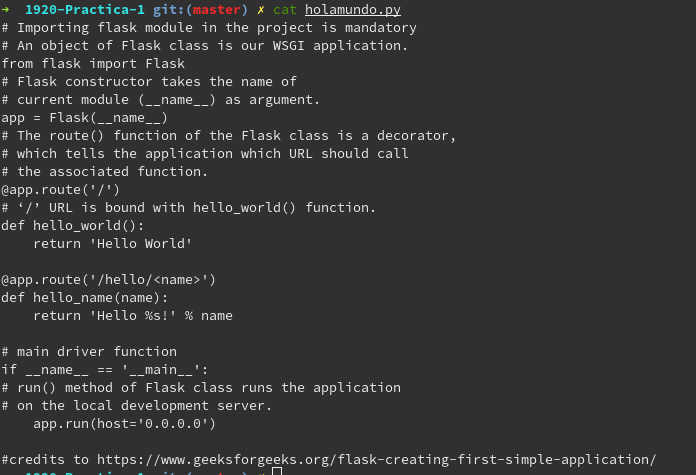
\includegraphics[width=0.7\textwidth]{img/img1.png} 
\end{center}
\end{description}
\item Definimos las dependencias en el archivo requirements.txt
\lstset{language=C, breaklines=true, basicstyle=\footnotesize}
\begin{lstlisting}[frame=single]
Flask
\end{lstlisting}
\item Podemos usar la imagen de python3 existente en los repositorios de docker, y modificarla anadiendo la aplicacion que hemos desarrollado. Para ello podemos crear un fichero Dockerfile que nos automatiza la creacion de una imagen modificada:

\begin{center}
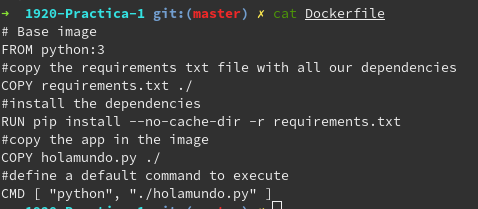
\includegraphics[width=0.7\textwidth]{img/img2.png} 
\end{center}
\item Este fichero indica que docker tiene que descargar la imagen python en su tercera versión y tiene que añadir el fichero requirements a la carpeta de usuario de la imagen. Docker nos ofrece un lenguaje de scripting para automatizar la creacion de imagenes.
\lstset{language=C, breaklines=true, basicstyle=\footnotesize}
\begin{lstlisting}[frame=single]
docker build -t holamundo-flask .
docker run -p 8020:80 holamundo-flask
\end{lstlisting}
\begin{center}
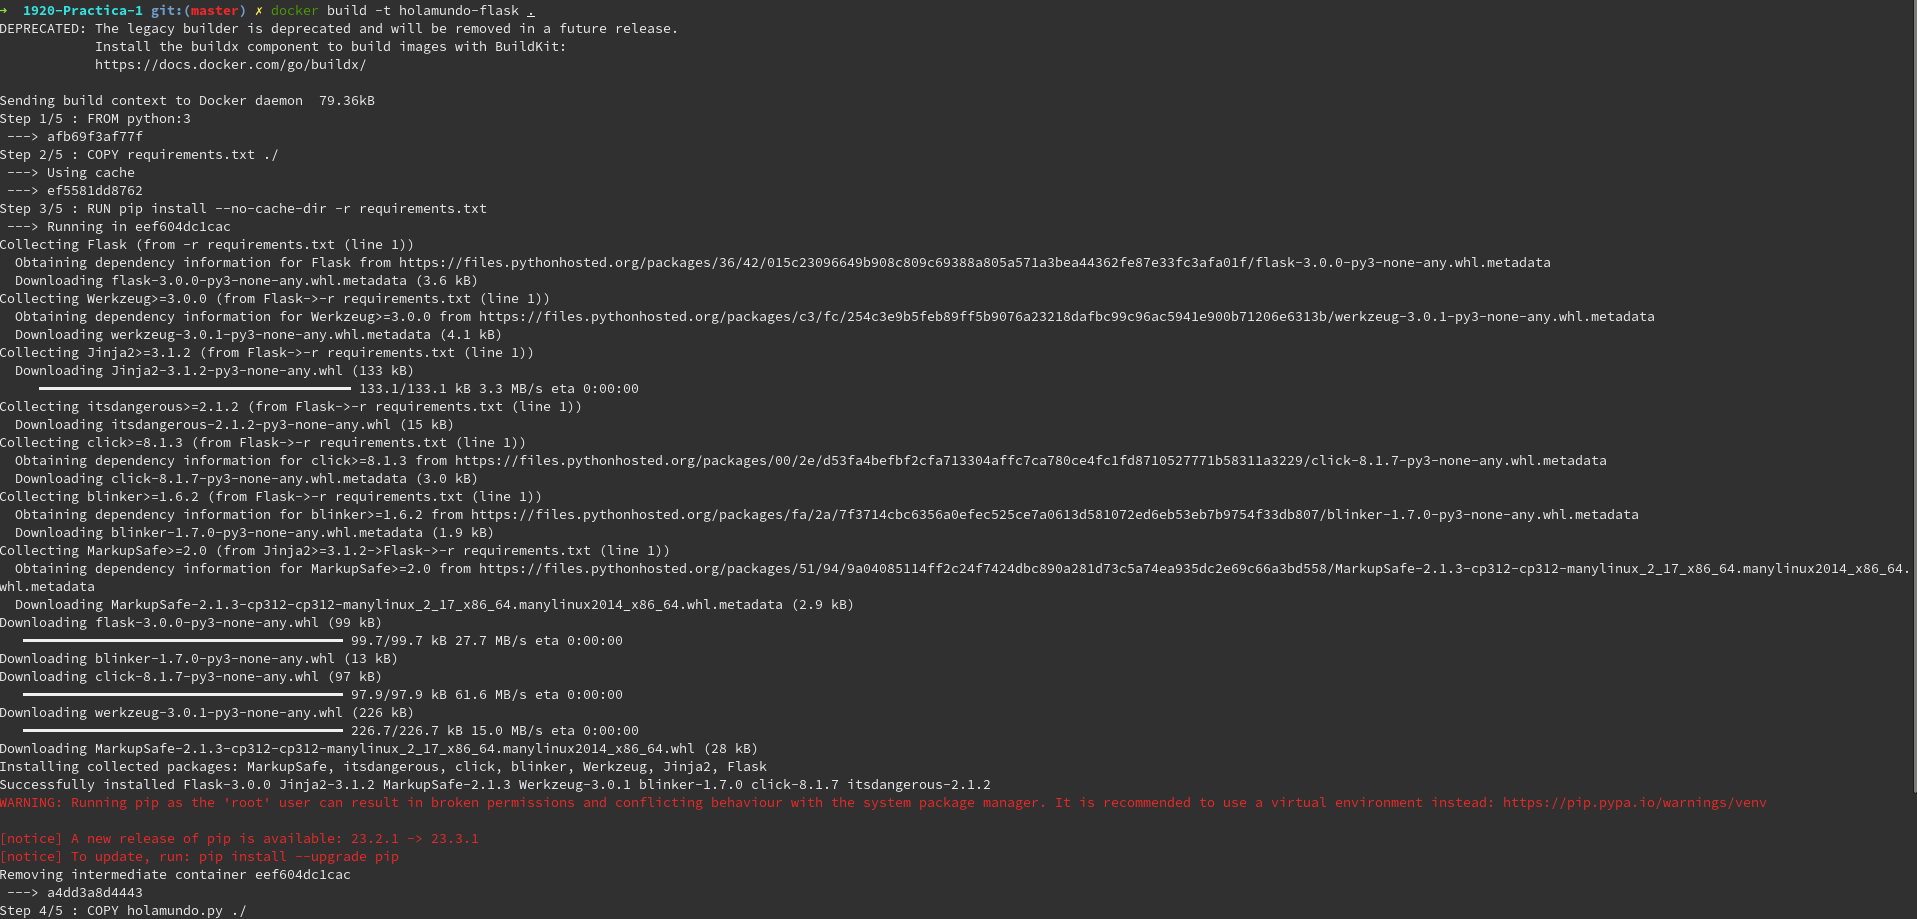
\includegraphics[width=\textwidth]{img/img3.png} 
\end{center}
\begin{center}
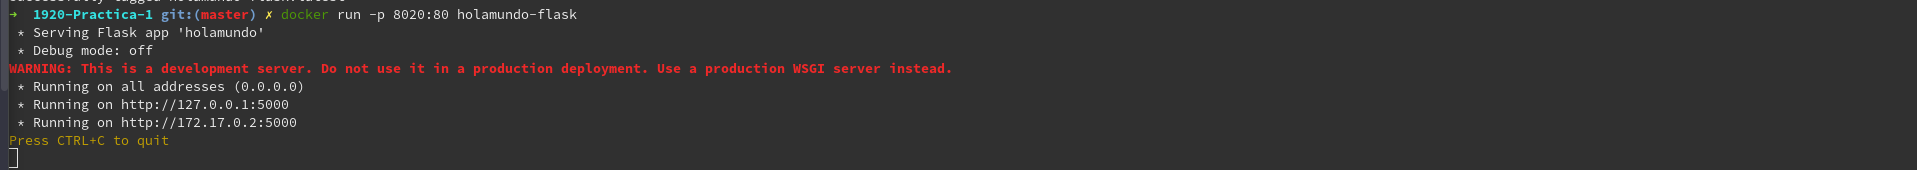
\includegraphics[width=\textwidth]{img/img4.png} 
\end{center}

\end{enumerate}



\newpage
\textbf{Parte 2}. Desplegar la aplicación web en una máquina virtual usando Vagrant. Para ello:

\begin{enumerate}
\item Instale Vagrant siguiendo las \href{https://1984.lsi.us.es/wiki-egc/index.php/Despliegue_de_aplicaciones:_M%C3%A1quinas_virtuales_22-23}{instrucciones de la siguiente página:}

\begin{description}
\item Intalación:
\lstset{language=C, breaklines=true, basicstyle=\footnotesize}
\begin{lstlisting}[frame=single]
sudo apt update
sudo apt install vagrant ansible virtualbox

//Para probar que funciona
vagrant init ubuntu/trusty32
vagrant up
#Suele tardar varios minutos
vagrant ssh -c 'hostnamectl'   
#Comparar que devuelve el comando con respecto a ejecutar hostnamectl en local
vagrant destroy #Para eliminar la imagen y liberar espacio
\end{lstlisting}


\end{description}
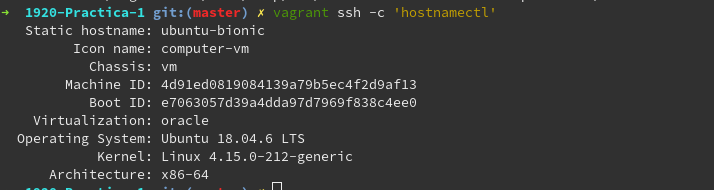
\includegraphics[width=\textwidth]{img/img5.png} 


\item Virtualize la aplicación (crea una máquina virtual y ejecútela) siguiendo las \href{https://1984.lsi.us.es/wiki-egc/index.php/Ejercicio_3:_Encapsulado_y_aprovisionamiento_de_una_app_en_Vagrant_21-22}{instrucciones de la
siguiente página:}
\begin{description}
\item Encapsulado y aprovisionamiento de una app
\item Creamos un Vagrantfile
\lstset{language=C, breaklines=true, basicstyle=\footnotesize}
\begin{lstlisting}[frame=single]
Vagrant.configure("2") do |config|
	config.vm.box = "ubuntu/bionic64"
  	config.vm.provision "shell", inline: "sudo apt-get update && sudo apt-get install -y docker.io"
  	config.vm.network "forwarded_port", guest: 80, host: 8080, host_ip: "127.0.0.1"
end
\end{lstlisting}
\item Creamos nuestra forma de aprovisionar (de momento con un script bash)
\lstset{language=C, breaklines=true, basicstyle=\footnotesize}
\begin{lstlisting}[frame=single]
sudo apt update
sudo apt upgrade -y
sudo apt install -y git python3 python3-pip screen 
git clone https://github.com/EGCETSII/1920-Practica-1.git
cd 1920-Practica-1
pip3 install -r requirements.txt 
screen -m -d python3 holamundo.py
\end{lstlisting}
\item vagrant up

\end{description}

\end{enumerate}

\begin{center}
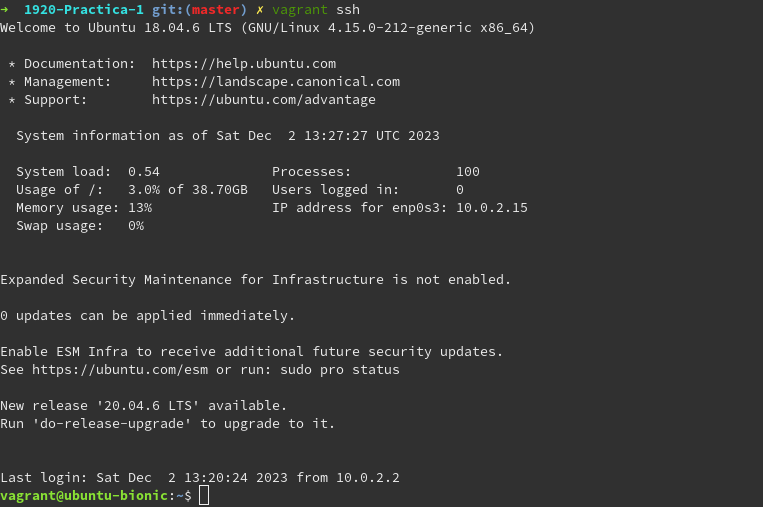
\includegraphics[width=\textwidth]{img/img6.png} 
\end{center}
\begin{center}
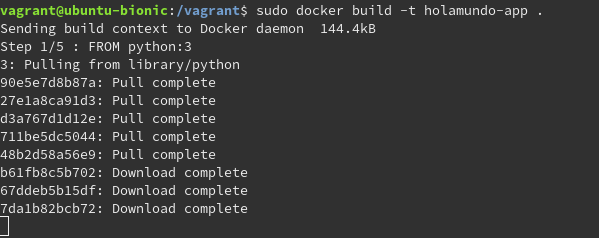
\includegraphics[width=\textwidth]{img/img7.png} 
\end{center}
\begin{center}
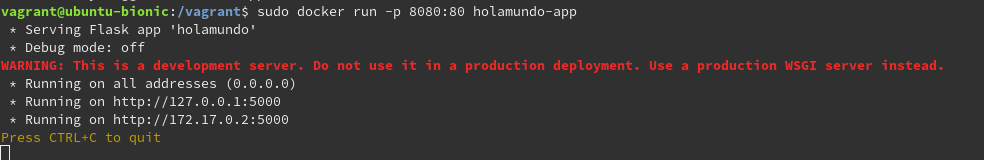
\includegraphics[width=\textwidth]{img/img8.png} 
\end{center}























\end{document}